% Copyright (c) 2022 by Lars Spreng
% This work is licensed under the Creative Commons Attribution 4.0 International License. 
% To view a copy of this license, visit http://creativecommons.org/licenses/by/4.0/ or send a letter to Creative Commons, PO Box 1866, Mountain View, CA 94042, USA.

%~~~~~~~~~~~~~~~~~~~~~~~~~~~~~~~~~~~~~~~~~~~~~~~~~~~~~~~~~~~~~~~~~~~~~~~~~~~~~~
% You can add your packages and commands to the loadslides.tex file. 
% The files in the folder "styles" can be modified to change the layout and design of your slides.
% I have included examples on how to use the template below. 
% Some of it these examples are taken from the Metropolis template.
%~~~~~~~~~~~~~~~~~~~~~~~~~~~~~~~~~~~~~~~~~~~~~~~~~~~~~~~~~~~~~~~~~~~~~~~~~~~~~~


\documentclass[
14pt,notheorems,hyperref={pdfauthor=whatever}
]{beamer}
\graphicspath{ {images/} }


% Copyright (c) 2022 by Lars Spreng
% This work is licensed under the Creative Commons Attribution 4.0 International License. 
% To view a copy of this license, visit http://creativecommons.org/licenses/by/4.0/ or send a letter to Creative Commons, PO Box 1866, Mountain View, CA 94042, USA.

%~~~~~~~~~~~~~~~~~~~~~~~~~~~~~~~~~~~~~~~~~~~~~~~~~~~~~~~~~~~~~~~~~~~~~~~~~~~~~~
% Add your packages and commands to this file
%~~~~~~~~~~~~~~~~~~~~~~~~~~~~~~~~~~~~~~~~~~~~~~~~~~~~~~~~~~~~~~~~~~~~~~~~~~~~~~

%~~~~~~~~~~~~~~~~~~~~~~~~~~~~~~~~~~~~~~~~~~~~~~~~~~~~~~~~~~~~~~~~~~~~~~~~~~~~~~
\RequirePackage{palatino}
\RequirePackage[utf8]{inputenc}
\RequirePackage[T1]{fontenc}
% Styles
\usefonttheme{serif}
\usepackage{xfrac}
\usepackage{styles/elegantmacros}
\usefolder{styles}
\usetheme[style=blue]{elegant}
% PDF import
\usepackage{pdfpages}

\newcommand{\makepart}[1]{ % For convenience
\part{#1} \frame{\partpage}
}

%~~~~~~~~~~~~~~~~~~~~~~~~~~~~~~~~~~~~~~~~~~~~~~~~~~~~~~~~~~~~~~~~~~~~~~~~~~~~~~

%~~~~~~~~~~~~~~~~~~~~~~~~~~~~~~~~~~~~~~~~~~~~~~~~~~~~~~~~~~~~~~~~~~~~~~~~~~~~~~
% Figures
\RequirePackage{booktabs}
\RequirePackage{colortbl}
\RequirePackage{ragged2e}
\RequirePackage{schemabloc}
%\RequirePackage{natbib}
\RequirePackage{caption}
\RequirePackage{subcaption}
\RequirePackage{tabularx}
\RequirePackage{array}
\RequirePackage{multirow}
\RequirePackage{multicol}
\RequirePackage{outlines}
\usepackage[
  style=authoryear, 
]{biblatex}
\addbibresource{references.bib}
\newcolumntype{Y}{>{\centering\arraybackslash}X}

%~~~~~~~~~~~~~~~~~~~~~~~~~~~~~~~~~~~~~~~~~~~~~~~~~~~~~~~~~~~~~~~~~~~~~~~~~~~~~~

%~~~~~~~~~~~~~~~~~~~~~~~~~~~~~~~~~~~~~~~~~~~~~~~~~~~~~~~~~~~~~~~~~~~~~~~~~~~~~~
% Figures
\RequirePackage{wrapfig}
\RequirePackage{pgfplots}
\RequirePackage{graphicx}
\RequirePackage{adjustbox}
\RequirePackage{environ}
\pgfplotsset{compat=1.18}

\makeatletter
\newsavebox{\measure@tikzpicture}
\NewEnviron{scaletikzpicturetowidth}[1]{%
  \def\tikz@width{#1}%
  \def\tikzscale{1}\begin{lrbox}{\measure@tikzpicture}%
  \BODY
  \end{lrbox}%
  \pgfmathparse{#1/\wd\measure@tikzpicture}%
  \edef\tikzscale{\pgfmathresult}%
  \BODY
}
\makeatother
%~~~~~~~~~~~~~~~~~~~~~~~~~~~~~~~~~~~~~~~~~~~~~~~~~~~~~~~~~~~~~~~~~~~~~~~~~~~~~~

%~~~~~~~~~~~~~~~~~~~~~~~~~~~~~~~~~~~~~~~~~~~~~~~~~~~~~~~~~~~~~~~~~~~~~~~~~~~~~~
% Maths 
\RequirePackage{textcomp}
\RequirePackage{amsmath} 
\RequirePackage{amsthm}
\RequirePackage{mathtools}
%\RequirePackage{bbm}
%\RequirePackage{algorithm}
%\RequirePackage[osf,sc]{mathpazo}
%\RequirePackage{pifont}
%\newcommand{\xmark}{\ding{55}}%
%\numberwithin{equation}{section}
\DeclareMathOperator*{\argmax}{arg\,max}
\DeclareMathOperator*{\argmin}{arg\,min}

\setbeamertemplate{theorems}[numbered] % to number

\theoremstyle{definition}
\newtheorem{fact}{Fact}[section]
\newtheorem{examp}{Example}[section]

\theoremstyle{plain}
\newtheorem{definition}{Definition}[section]
\newtheorem{proposition}{Proposition}
\newtheorem{theorem}{Theorem}
\newtheorem{assumption}{Assumption}

\providecommand{\H}{\mathscr{H}}      
\providecommand{\E}{\mathbb{E}}
\makeatletter
\def\munderbar#1{\underline{\sbox\tw@{$#1$}\dp\tw@\z@\box\tw@}}
\makeatother

%~~~~~~~~~~~~~~~~~~~~~~~~~~~~~~~~~~~~~~~~~~~~~~~~~~~~~~~~~~~~~~~~~~~~~~~~~~~~~~
 % Loads packages and some defined commands

\title[
% Text entered here will appear in the bottom middle
]{Theory of Financial Markets}

\subtitle{BUS 891 - Fall 2023}

\author[
% Text entered here will appear in the bottom left corner
]{
    Eduardo Schwartz 
}
\institute{
    Ryan Beedie Chair in Finance, \\
    Simon Fraser University}
\date{\today}

\AtBeginSection[]{
  \begin{frame}{Topic \thesection}
  \vfill
  \centering
    \usebeamerfont{title}\insertsectionhead\par%
  \vfill
  \end{frame}
}

\begin{document}

% Generate title page
{
\setbeamertemplate{footline}{} 
\begin{frame}
  \titlepage
\end{frame}
}
\addtocounter{framenumber}{-1}

%% FRAME Table of Contents
\begin{frame}[plain,noframenumbering]{Theory of Financial Markets}
    \setcounter{tocdepth}{2}
        \tableofcontents[sections={1-3}]
\end{frame}
\begin{frame}[plain,noframenumbering]{Theory of Financial Markets (cont.)}
    \setcounter{tocdepth}{2}
        \tableofcontents[sections={4-9}]
\end{frame}
\begin{frame}[plain,noframenumbering]{Theory of Financial Markets (cont.)}
    \setcounter{tocdepth}{2}
        \tableofcontents[sections={10-14}]
\end{frame}
\begin{frame}[plain,noframenumbering]{Theory of Financial Markets (cont.)}
    \setcounter{tocdepth}{2}
        \tableofcontents[sections={15-20}]
        \vspace{166px}
\end{frame}

%%%%%%%%%%%%%%%%%%%%%%%%%%%%%%%%%%%%%%%%%%%%%%%%%%%%%
%%%%%%%%% TOPIC 1  Expected Utility and RA %%%%%%%%%%
%%%%%%%%%%%%%%%%%%%%%%%%%%%%%%%%%%%%%%%%%%%%%%%%%%%%%
\section{Intro to Expected Utility \& Risk Aversion}
\begin{frame}
\alert{\textbf{Basic Ideas}}
\begin{itemize}
    \item St. Petersburg Paradox
    \item Expected Utility Theorem
    \item Risk Aversion
    \item Absolute and Relative Risk Aversion
    \item Useful Utility Functions
\end{itemize} 
\end{frame}


\subsection{St. Petersburg Paradox}

\begin{frame}
Coin flipping game: toss a coin, and continue to do so until it lands "heads".
\begin{table}
    %\caption{}
    \begin{tabular}{@{} lr @{}}
      \toprule
      Payout & Probability\\
      \midrule
      \$1 if “heads” the first time (H) & $\sfrac{1}{2}$\\
      \$2 if “heads” the second time (TH) & $\sfrac{1}{4}$\\
      \$4 if “heads” the third time (TTH) & $\sfrac{1}{8}$\\
      ...\\
      \$2 if “heads” the $i^{th}$ time (TT...TH) & $(\sfrac{1}{2})^i$\\
      \bottomrule
    \end{tabular}
\end{table}
\end{frame}

\begin{frame}
\begin{itemize}
    \item Poll: How much are you willing to pay to play this game?
\end{itemize}
\hfill \break
\begin{enumerate}
\setlength{\itemindent}{.5in}
    \item Not more than \$2
    \item Not more than \$5
    \item Not more than \$10
    \item Not more than \$20
    \item Not more than \$100
\end{enumerate}
\end{frame}

\begin{frame}
Expected payoff:
\begin{align*}
    \bar{x} &= \sum_{i=1}^{\infty}p_i x_i = \frac{1}{2}\cdot1 + \frac{1}{4}\cdot2+ \frac{1}{8}\cdot4 + ... + (\frac{1}{2})^i \cdot2^{i-1} + ...\\
    &= \frac{1}{2} + \frac{1}{2} + \frac{1}{2} + ... + \frac{1}{2} + ... = \frac{1}{2} (1+1+1+...+1+...) = \infty
\end{align*}
The “paradox” is that the expected value is infinity, but most individuals would pay only a moderate amount to play this game.
\end{frame}


\subsection{Expected Utility Theorem}

\begin{frame}
Bernoulli (1738) provided and explanation of the paradox: individuals do not maximize expected value, but \textbf{expected utility}:
\[ V \equiv E[u(\tilde{x})] = \sum_{i=1}^n p_i u(x_i)\]
The maximum they would pay is an amount that has the same utility as the expected utility of this lottery (Certainty Equivalent). $V=u(CE)$\\
The first complete axiomatic development of expected utility is due to von Neumann and Morgenstern (1944).
\end{frame}

\begin{frame}
Axioms of Rational Behaviour\\
\hfill \break
1. \textit{Completeness}: there exists a preference ordering over all risky prospects which is complete. i.e. for any two gambles x and y\\
\begin{center}
    $x \succ y$ or $x \prec y$ or $x \sim y$
\end{center}
\begin{figure}[ut1]
    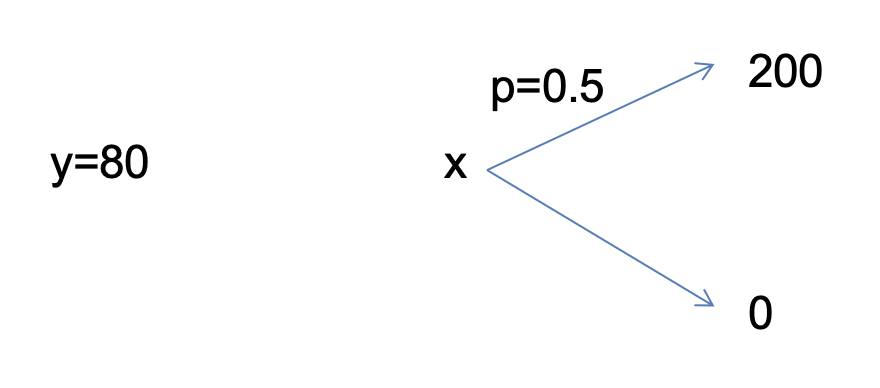
\includegraphics[width=0.5\textwidth]{L1UT1}
    \centering
\end{figure}
\end{frame}

\begin{frame}
Axioms of Rational Behaviour\\
\hfill \break
2. \textit{Transitivity}: the preference ordering is transitive\\
\begin{center}
    if $x \succ y$ and $y \succ z \implies x \succ z$\\
    if $x \sim y$ and $y \sim z \implies x \sim z$
\end{center}
\begin{figure}[ut2]
    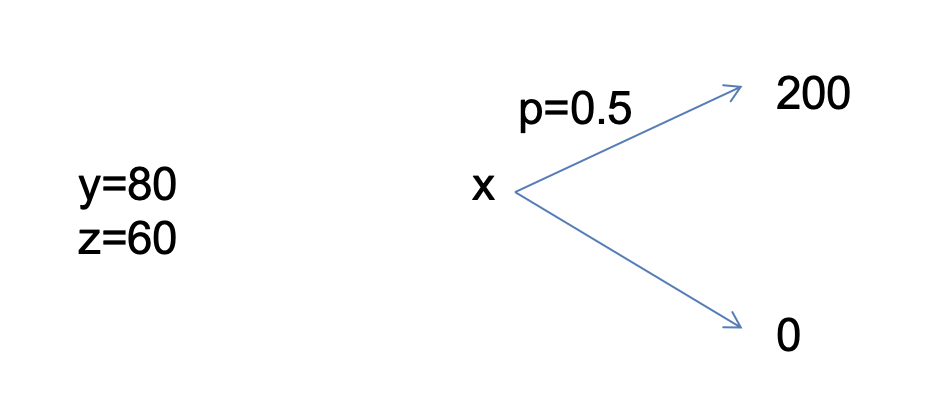
\includegraphics[width=0.5\textwidth]{L1UT2}
    \centering
\end{figure}
\end{frame}

\begin{frame}
Axioms of Rational Behaviour\\
\hfill \break
3. \textit{Independence}: Let $g(x,z;p)$ represent a gamble with probability p of paying x and (1-p) of paying z\\
\begin{figure}[ut3]
    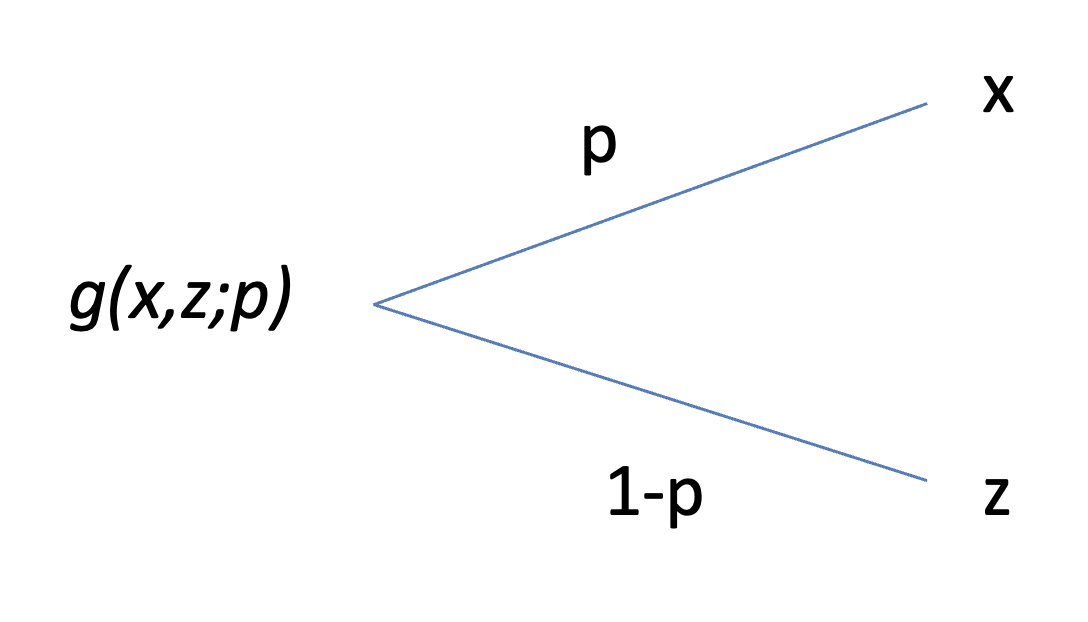
\includegraphics[width=0.4\textwidth]{L1UT3}
    \centering
\end{figure}
\begin{align*}
    &\textrm{if } x \sim y\\
    &\textrm{then } g(x,z;p) \sim g(y,z;p)
\end{align*}
\end{frame}

\begin{frame}
Axioms of Rational Behaviour\\
\hfill \break
4. \textit{Continuity}: If $x \succsim y \succsim z$ then there exists a probability p (unique unless $x \sim y \sim z$) such that $y \sim g(x,z;p)$\\
\begin{figure}[ut4]
    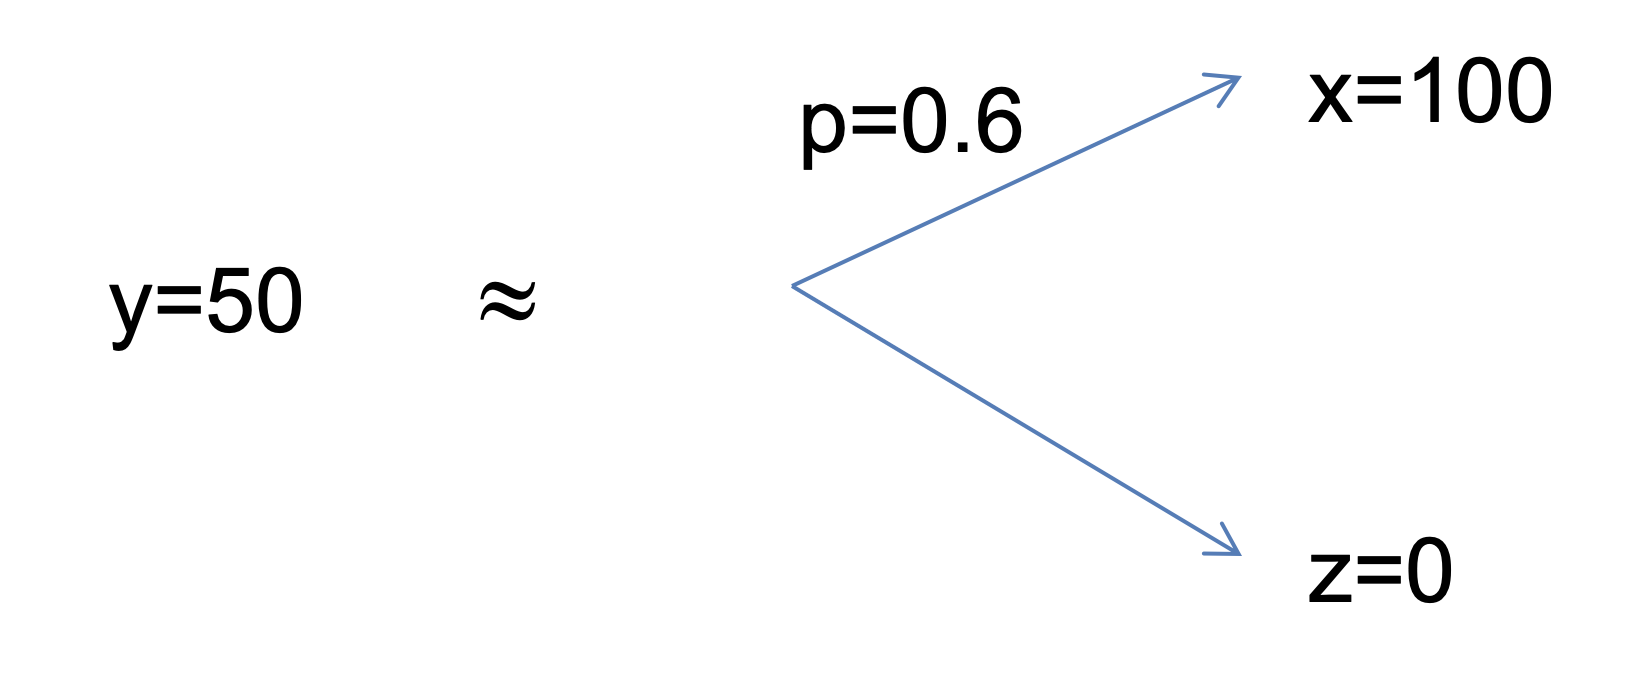
\includegraphics[width=0.5\textwidth]{L1UT4}
    \centering
\end{figure}
\end{frame}

\begin{frame}
Axioms of Rational Behaviour\\
\hfill \break
5. \textit{Dominance}: If $x \succ y \succ z$ and $x \succ t \succ z$, $y \sim g(x,z;p_1)$ and $t \sim g(x,z;p_2)$\\
\begin{center}
    then $p_1 > p_2 \implies y \succ t$\\
    and $p_1 = p_2 \implies y \sim t$\\
\end{center}
\begin{figure}[ut4]
    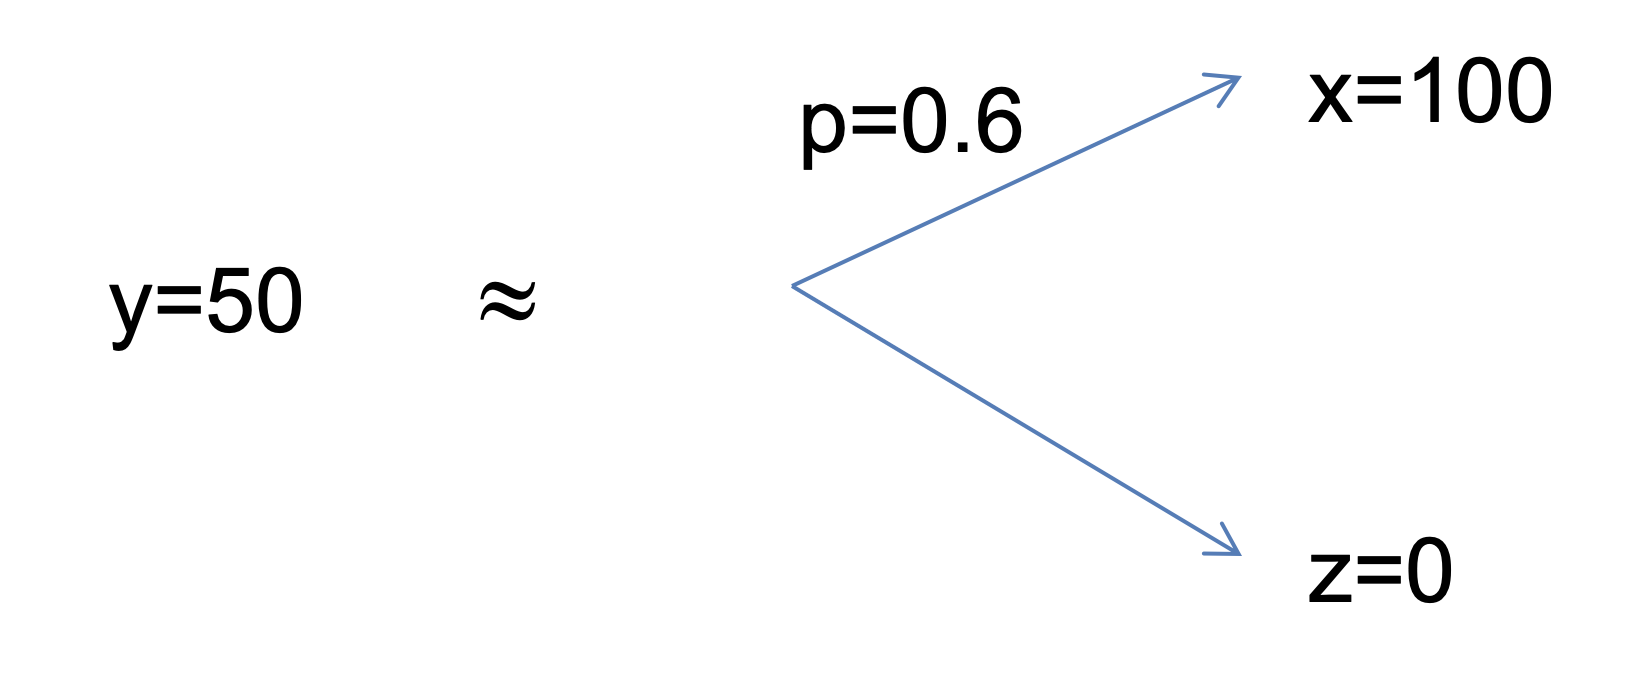
\includegraphics[width=0.5\textwidth]{L1UT4}
    \centering
\end{figure}
\end{frame}

\begin{frame}
Rational Preferences Under Uncertainty\\
\hfill \break
\textbf{Existence}: A preference ordering on risky prospects which satisfy these rationality requirements can be represented by a utility function u defined over the set of outcomes in the sense that\\
\hfill \break
\begin{center}
    $E[u(x)] \geq E[u(y)]$\\
    $iff\;x \succsim y$\\
\end{center}
\end{frame}

\begin{frame}
Rational Preferences Under Uncertainty\\
\hfill \break
\textbf{Uniqueness}: u(x) is unique up to a positive linear transformation.\\
\hfill \break
If u(x) is a utility function, so is $v(x)=au(x)+b$ with $a>0$ \\
\begin{center}
    $E[v(x)] \geq E[u(y)]$\\
    $E[au(x)+b] \geq E[au(y)+b]$\\
    $aE[u(x)]+b \geq aE[u(y)]+b$\\
    $E[u(x)] \geq E[u(y)]$\\
\end{center}
\end{frame}


\subsection{Risk Aversion}

\begin{frame}
Concave utility function for wealth: $u''<0$\\
\hfill \break
Feel more “pain” to lose \$100 than “pleasure” to win \$100. Decreasing marginal utility of money\\
\hfill \break
($u'>0$ since more is preferred to less!)\\
\end{frame}

\begin{frame}
Investor will not trade \$100 for sure for 50/50 chance of getting \$200 or nothing\\
\hfill \break
With concave utility:\\
\begin{center}
    $u(100) > 0.5 u(200) + 0.5 u(0)$\\
\end{center}
\end{frame}

\begin{frame}
Risk Averse\\
\hfill \break
\begin{itemize}
    \item Investor will not trade \$100 for sure for 50/50 chance of getting \$200 or nothing
    \item With concave utility:
\end{itemize}
\begin{center}
    $u(100) > 0.5 u(200) + 0.5 u(0)$\\
\end{center}
TODO: risk-aversion image
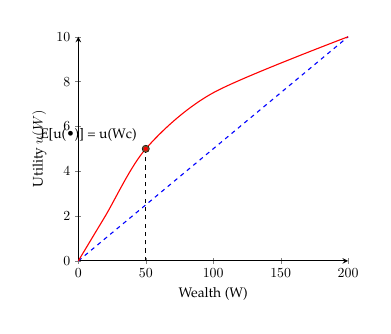
\begin{tikzpicture}[scale=0.5]
\begin{axis}[axis lines=left,xlabel=Wealth (W),ylabel=Utility $u(W)$,xmin=0, xmax=200,ymin=0, ymax=10,xtick={0,50,100,150,200},clip=false,domain=0:200,samples=100,thick,]
\addplot+[mark=none, dashed] {x/200*10};
\addplot+[mark=none,smooth] coordinates {(0,0) (20,2) (50,5) (100,7.5) (200,10)};
\addplot+[only marks, mark=*, mark options={fill=red}] coordinates {(50,5)};
\addplot+[mark=none, dashed] coordinates {(50,0) (50,5)};
\node[label={150:{E[u(•)] = u(Wc)}},circle,fill,inner sep=2pt] at (axis cs:50,5) {};
\end{axis}
\end{tikzpicture}
\end{frame}

\begin{frame}
Risk Neutral\\
\hfill \break
\begin{itemize}
    \item Linear utility function for wealth: $u''=0$
\end{itemize}
TODO: risk-neutral image
\hfill \break
Investor maximizes expected wealth\\
\end{frame}

\begin{frame}
Risk Seeking\\
\hfill \break
\begin{itemize}
    \item Convex utility function for wealth: $u''>0$
\end{itemize}
TODO: risk-seeking image
\hfill \break
Gambling?\\
\end{frame}

\begin{frame}
\textbf{Certainty Equivalent for Complex Gambles ($W_c$)}\\
\begin{center}
    $u(W_c) > E[u(complex\;gamble)]$\\
\end{center}
\begin{center}
    Amount you would accept for certain instead of the gamble.
\end{center}
\hfill \break
If $\bar{W}$ is the expected outcome:\\
\begin{enumerate}
\setlength{\itemindent}{.5in}
    \item risk averse if $W_c < \bar{W} \impliedby u''<0$  concave
    \item risk neutral if $W_c = \bar{W} \impliedby u''=0$  linear
    \item risk seeker if $W_c > \bar{W} \impliedby u''>0$  convex
\end{enumerate}
\end{frame}

\begin{frame}
Risk Averse Certainty Equivalent\\
TODO: certainty equivalent image
\end{frame}

\subsection{Absolute and Relative Risk Aversion}

\begin{frame}
\textbf{Measures of Risk Aversion}\\
\hfill \break
Size of  $u''(W)<0$  is not meaningful (unique up to a positive linear transformation),  $u'(W)>0$ more is preferred to less.\\
\begin{itemize}
    \item Absolute Risk Aversion $\;A(W) = -\frac{u''(W)}{u'(W)}$\\
    \item Relative Risk Aversion $\;\;R(W) = -\frac{Wu''(W)}{u'(W)} = W\cdot A(W)$\\
\end{itemize}
\hfill \break
Independent of positive linear transformation of the utility fn.
\begin{center}
    $v(W)=au(W)+b$, with $a>0$\\
\end{center}
Allows comparisons between individuals.\\
\end{frame}

\begin{frame}
\textbf{Measures of Risk Aversion}\\
\hfill \break
\begin{align*}
    v(W)&=au(W)+b, a>0\\
    v'(W)&=au'(W)>0\\
    v''(W)&=au''(W)<0\\
\end{align*}
\begin{align*}
    A(W)&=-\frac{u''(W)}{u'(W)}=-\frac{v''(W)}{v'(W)}>0\\
    R(W)&=-\frac{Wu''(W)}{u'(W)}=-\frac{Wv''(W)}{v'(W)}>0\\
\end{align*}
\end{frame}

\subsection{Useful Utility Functions}
\begin{frame}
\textbf{Exponential}: constant absolute risk aversion\\
\begin{align*}
    u(W)&=-\frac{1}{a}e^{-aW} \textit{ with } a>0\\
    u'(W)&=e^{-aW}>0\\
    u''(W)&=-ae^{-aW}<0\\
    A(W)&=-\frac{u''(W)}{u'(W)} = a\\
\end{align*}
TODO: exponential ut fn
\end{frame}

\begin{frame}
\textbf{Power}: constant relative risk aversion\\
\begin{align*}
    u(W)&=\frac{W^\gamma}{\gamma} \textit{ for } \gamma<1, \gamma\neq0\\
    u'(W)&=W^{\gamma-1}>0\\
    u''(W)&=(\gamma-1)W^{\gamma-2}<0\\
    R(W)&=-\frac{Wu''(W)}{u'(W)} = 1-\gamma = c > 0, \gamma < 1 \;\; u(W)=\frac{W^{1-c}}{1-c}\\
\end{align*}
TODO: power ut fn
\end{frame}

\begin{frame}
\textbf{Log}: also constant relative risk aversion\\
\begin{align*}
    u(W)&=\ln{W} (\gamma=0)\\
    u'(W)&=\frac{1}{W}>0\\
    u''(W)&=-\frac{1}{W^2}<0\\
    R(W)&=-\frac{Wu''(W)}{u'(W)}=1\\
\end{align*}
\end{frame}

\begin{frame}
\textbf{Quadratic}\\
\begin{align*}
    u(W)&=W-\frac{1}{2}bW^2 \textit{\;\;for } 0\leq W\leq \frac{1}{b}\\
    u'(W)&=1-bW>0 \textit{\;\;for } 0\leq W\leq \frac{1}{b}\\
    u''(W)&=-b<0\\
    A(W)&=-\frac{b}{1-bW} \textit{\;\;increasing with W (not good)}\\
\end{align*}
\end{frame}

\begin{frame}
Expected utility max. and mean variance analysis are equivalent when...\\
\hfill \break
\begin{outline}
    \1 Utility functions are quadratic
    \begin{align*}
        u(W)&=W-\frac{1}{2}bW^2\\
        E[u(W)]&=\Bar{W}-\frac{1}{2}b[\Bar{W}^2+Var(W)]
    \end{align*}
    \1 Distributions of returns are joint normal
        \2 Normal is completely defined by mean and variance
        \2 Additive
        \2 Indifference curves (constant Eu) can be written in terms of mean and s.d. only
    \1 Be careful when distributions are not normal (options)
\end{outline}
\end{frame}

\begin{frame}
Indifference Curves (for risk averse)\\
\hfill \break
A and B have the same expected utility
\end{frame}

\begin{frame}
Expected Utility - Example
\hfill \break
\begin{outline}
    \1 Your current wealth is \$100,000.
    \1 You want to purchase a homeowner’s insurance policy to cover potential loss due to fire.
    \1 You estimate that the probability of fire is 10\%
    \1 If your house is damaged by fire your loss would be \$60,000. 
    \1 You have determined that your utility of wealth is $U(W) = \sqrt{W}$. 
    \1 What is the maximum amount you would be willing to pay to fully insure against possible losses due to fire?
\end{outline}
\end{frame}

\begin{frame}
Expected Utility - Solution
\hfill \break
\begin{outline}
    \1 Let us assume that you will at the most be willing to pay \$D\break
    \1 If you buy insurance your wealth is \$(100,000 – D) for sure.\break
    \1 If you do not buy insurance there is a 10\% chance that you will end with a wealth of \$40,000 and a 90\% chance that you will end with a wealth of \$100,000\break
\end{outline}
\end{frame}

\begin{frame}
Expected Utility - Solution\\
TODO: img
\end{frame}

\begin{frame}
Expected Utility - Solution
\hfill \break
\begin{outline}
    \1 We defined certainty equivalent, $W_c$  as that amount of wealth which makes you indifferent between this wealth and a gamble\break
    \1 That is $U(W_c) = E[U]$
    \begin{align*}
        U(100,000 - D) &= 0.1\cdot U(40,000) + 0.9\cdot U(100,000)\\
        \sqrt(100000-D) &= 0.1\sqrt{40,000} + 0.9\sqrt{100,000}\\
        D &= 7,215.80 > 6,000 \textit{ expected loss }\\
    \end{align*}
\end{outline}
\end{frame}


%%%%%%%%%%%%%%%%%%%%%%%%%%%%%%%%%%%%%%%%%%%%%%%%%%%%%
%%%%%%%%%%%%% TOPIC 2  Utility Theorem %%%%%%%%%%%%%%
%%%%%%%%%%%%%%%%%%%%%%%%%%%%%%%%%%%%%%%%%%%%%%%%%%%%%
\section{Utility Theory}  % TOPIC 2: Utility Theory

\begin{frame}
Rational "preferences" under uncertainty (over consumption hurdles):\\
\begin{outline}
    \1 Completeness
    \1 Transitivity
    \1 Continuity
    \1 Monotonicity (more is preferred to less)
\end{outline}
Ordinal utility fn: any positive transformation preserves the same ordering\\
\end{frame}

\begin{frame}
Rational "preferences" under uncertainty:\\
\hfill \break
Existence and uniqueness theorems based on certain rationality requirements (axioms of rational behaviour).\\
\hfill \break
Even though these axioms have been challenged there is no theory competing with this:\\
\begin{outline}
    \1 measurable or Von Neumann-Morgenstern utility fn.
      \2 "Preferences over gambles"
\end{outline}
\hfill \break
Let $S$ be the set of all risky prospects  payoff distributions).\\
\end{frame}

\subsection{Expected Utility Theorem}

\begin{frame}
Let $S$ be the set of all risky prospects  payoff distributions).\\
\hfill \break
\underline{\textbf{Expected Utility Theorem}}: A preference ordering on $S$ which satisfies certain rationality requirements (A1-A5) can be represented by a utility function $u$ defined on the set of outcomes in the sense that:\\
\hfill \break
\textit{Existence}
\begin{align*}
    E[u(x)] \geq& E[u(y)]\\
    x, y \; \epsilon& \; S\\
    \textit{ iff } x \succsim & \; y\\
\end{align*}
\end{frame}

\begin{frame}
If $u(x)$ is a utility function, so is $au(x)+b\textit{, }a>0$. That is, $u(x)$ is unique up to a positive linear transformation. \\
\hfill \break
\textit{Uniqueness}
\begin{align*}
    E[u(x)] =& \sum_i u(x)_i p(x_i)\\
    =& \int_{-\infty}^\infty u(x)f(x)dx\\
    =& \int_{-\infty}^\infty u(x)dF(x)\\
    F(x) =& Pr\{X \leq x\}\\
    f(x) =& \frac{dF(x)}{dx}\\
\end{align*}
\end{frame}

\subsection{Axioms}

\begin{frame}
Axioms governing investors' behavior\\
\hfill \break
\textbf{A1 (Completeness)}: There exists a preference ordering over all risky prospects which is complete.\\
\hfill \break
ie. For any two gambles $x,y$
\hfill \break
\begin{align*}
    x &\succ y\\
    x &\prec y\\
    x &\sim y\\
\end{align*}
\end{frame}

\begin{frame}
Axioms governing investors' behavior\\
\hfill \break
\textbf{A2 (Transitivity)}: The preference ordering is transitive\\
\hfill \break
\begin{align*}
    \textit{If }x &\succ y \textit{ and } y \succ z \implies x \succ z\\
    x &\sim y \textit{ and } y \sim z \implies x \sim z\\
\end{align*}
\end{frame}

\begin{frame}
Axioms governing investors' behavior\\
\hfill \break
\textbf{A3 (Independence)}: Let $g(x,z;p)$ represent a gamble with probability $p$ of paying $x$ and $(1-p)$ of paying $z$.\\
TODO: gamble img\\
\hfill \break
\begin{align*}
    \textit{If }x &\sim y\\
    \textit{Then }g(x,y;p) &\sim g(y,z;p)\\
\end{align*}
\end{frame}

\begin{frame}
Axioms governing investors' behavior\\
\hfill \break
\textbf{A4 (Continuity)}: If $x \succsim y \succsim z$ then there exists a probability $p$ (unique unless $x \sim y \sim z$) such that\\
\hfill \break
\begin{align*}
    y &\sim g(x,z;p)\\
\end{align*}
\end{frame}

\begin{frame}
Axioms governing investors' behavior\\
\hfill \break
\textbf{A5 (Dominance)}:
\begin{align*}
    \textit{If }\;\;x \succsim y \succsim z,&\;\; x \succsim t \succsim z\\
    \textit{and }\;\;y \sim g(x,z;p_1),&\;\; t \sim g(x,z;p_2)\\
\end{align*}
\begin{align*}
    \textit{Then }\;\;p_1 > p_2 \implies& y \succ t\\
    \textit{and }\;\;p_1 = p_2 \implies& y \sim t\\
\end{align*}
\end{frame}

\subsection{Derivation}

\begin{frame}
\underline{\textbf{Derivation}}:\\
\hfill \break
Consider a set of (simple) gambles $g(M,m;h)$, that is, the payment $M$ with probability $h$ and $m<M$ with probability $1-h$.\\
From A4 (Continuity) we have $W_i\;\epsilon\;(m,M)$ such that\\
\[W_i \sim g(M,m;h(W_i))\]
\hfill \break
$W_i$ is the certainty equivalent of the gamble.
\end{frame}

\begin{frame}
We can construct the indifference set for $h=(0,1)$, (for a given individual)\\
TODO: indiff curve image\\
\[W_i = hM+(1-h)m\]
\hfill \break
For this preference function (concave) CE < Expected payoff of the gamble ($W_i<\bar{W_i}$)
\end{frame}

\begin{frame}
Consider a (complex) gamble with payoffs $X_i$ with probabilities $p_i$, $i=1,...,n$\\
TODO: complex gamble\\
By A4 (Continuity) we can find $h_i$ such that $X_i \sim g(M,m;h_i)$.\\
By A3 (Independence)\\
TODO: equivalence
\end{frame}

\begin{frame}
Consider a second (complex) gamble with outcomes $Y_i$ and probabilities $q_i$, $i=1,...,N$\\
Then this gamble is equivalent to $g(M,m;Q)$
for
\[Q \equiv \sum_{i=1}^N q_i\;h(Y_i)\;\;,\;\;Y_i\sim g(M,m;h(Y_i))\]
\begin{align*}
    \therefore \;\; \Tilde{X}&\sim g(M,m;H)\\
    \Tilde{Y}&\sim g(M,m;Q)\\
\end{align*}
From A5 (Dominance) $\Tilde{X} \succ \Tilde{Y}$ iff $H > Q$ ...
\end{frame}

\begin{frame}
...we can write the probabilities $h(X_i) = u(x)$\\
\[\therefore \;\; \Tilde{X}\succ\Tilde{Y}\;\; \textit{ iff }\;\; E[u(x)]>E[u(y)]\]
\begin{center}
    \textbf{This is the expect utility theorem}\\
\end{center}
\hfill \break
The same preference ordering can be obtained by:\\
\[v(x)=a\;u(x)+b \;\;\;\; a,b \textit{ constants; } a>0\]
$\implies$ unique up to a positive linear transformation.\\
(Note: Interpersonal comparisons of utility are not possible.)
\end{frame}

\begin{frame}
\[v(x)=a\;u(x)+b \;\;\;\; a,b \textit{ constants; } a>0\]
\hfill \break
\underline{\textbf{b}} determines the origin and \underline{\textbf{a}} determines the scale of the utility measures (but they don't change the preference ordering).\\
\hfill \break
This should not be surprising because the selection of $\$m$ and $\$M$ were an arbitrary two points in the utility function.
\end{frame}

\subsection{Certainty Equivalent}

\begin{frame}
Certainty equivalent $W_c$ for complex gambles:
\[W_c \sim g(M,m;H)\]
\[\textit{ie. } u(W_c) = E[u(\textit{complex gamble}]\]
\hfill \break
If $\bar{W}$ is the expected outcome, then the individual is said to be:
\begin{align*}
    \textit{risk-averse if } W_c &< \bar{W} \impliedby u''<0\\
    \textit{risk-neutral if } W_c &= \bar{W} \impliedby u''=0\\
    \textit{risk-seeking if } W_c &> \bar{W} \impliedby u''>0\\
\end{align*}
It is easy to show this by Taylor's Theorem...
\end{frame}

\begin{frame}
\begin{align*}
    \textit{risk-averse if } W_c &< \bar{W} \impliedby u''<0\\
    \textit{risk-neutral if } W_c &= \bar{W} \impliedby u''=0\\
    \textit{risk-seeking if } W_c &> \bar{W} \impliedby u''>0\\
\end{align*}
By Taylor's Theorem:
\begin{align*}
    E[u(W)] &= E[u(\bar{W}+(W-\bar{W}))]\\
    &= E[u(\bar{W})]+u'(\bar{W})(W-\bar{W})\\
    &\;\;\;+\frac{1}{2}u''(\bar{W}(1-\theta)+\theta W)(W-\bar{W})^2\;\;\textit{for some }\theta, 0 \leq \theta \leq 1\\
    \therefore \;\; E[u(W)]-E[u(\bar{W})] &= u(W_c)-u(\bar{W}) = \frac{1}{2}E[u''(\cdot)(W-\bar{W})^2\\
\end{align*}
\end{frame}

\subsection{Example}

\begin{frame}
TODO: add illustrated risk-* examples.
\end{frame}

%%%%%%%%%%%%%%%%%%%%%%%%%%%%%%%%%%%%%%%%%%%%%%%%%%%%%
%%%%%%%%%%%%%% TOPIC 3  Risk Aversion %%%%%%%%%%%%%%%
%%%%%%%%%%%%%%%%%%%%%%%%%%%%%%%%%%%%%%%%%%%%%%%%%%%%%
\section{Risk Aversion}
\begin{frame}
We will assume that decision makers maximize expected utility of terminal wealth (one period model). Expected Utility Theorem: Von Neumann-Morgenstern utility function existence and uniqueness (if axioms of rational behaviour hold).\\
\hfill \break
\underline{risk averse}: if unwilling to accept every actuarially fair and immediately resolved gamble.\\
\[\textit{ie. } u(W) > E[u(W+\hat{\varepsilon})]\]
\[\textit{for all gambles with $E[\hat{\varepsilon}]=0$ and $\sigma_\varepsilon^2 >0$}\]
\hfill \break
\underline{globally risk averse}: if risk averse at all levels of wealth.\\
\end{frame}

\begin{frame}
Theorem: A necessary and sufficient condition for (global) risk aversion is a utility function of wealth that is strictly concave.\\
\hfill \break
Proof: if $u(\cdot)$ is strictly concave at W by Jensen's inequality\\
\[ E[U(W+\tilde\varepsilon)] < U(E[W+\tilde\varepsilon]) = U(W)\]
\hfill \break
Actuarially Fair Gamble:\\
\[p\varepsilon_1+(1-p)\varepsilon_2 = 0\]
\[\varepsilon_1>0\;\;,\;\;\varepsilon_2<0\]
\end{frame}

\begin{frame}
Risk Averse\\
\hfill \break
\[ u(W)+\tilde\varepsilon)] < U(E[W+\tilde\varepsilon]) = U(W)\]
\begin{align*}
    u(W) &= u(p(W+\varepsilon_1)+(1-p)(W+\varepsilon_2))\\
    &> p u(W+\varepsilon_1)+(1-p)u(W+\varepsilon_2)
\end{align*}
TODO: add risk aversion concave function image\\
$\therefore$ risk averse $\implies$ concave utility function.\\
A reversal of these steps demonstrates that concave utility function $\implies$ risk averse.\\
\end{frame}

\begin{frame}
To avoid a gamble, a risk averse person would be willing to pay an \underline{insurance risk premium}, $\pi_i$ (used in economic analyses)\\
\hfill \break
1. $E[U(W+\tilde\varepsilon)] = U(W-\pi_i)$\\
\hfill \break
$W-\pi_i$: the certainty equivalent of gamble $W+\tilde\varepsilon$\\
To induce a risk averse investor to undertake a gamble, a \underline{compensatory} risk premium $\pi_C$ would have to be offered.\\
\hfill \break
2. $E[U(W+\pi_c+\tilde\varepsilon)] = U(W)$\\
\hfill \break
Used in financial applications, "extra" return expected on a riskier assets.\\
\hfill \break
The two premia are closely related but not identical. If utility function is smooth and risk is small, they are almost equal.\\
\end{frame}

\subsection{Measures of Risk Aversion}
\begin{frame}
The size of $u''(W)<0$ is not meaningful, $u'(W)>0$ more is preferred to less.\\
\hfill \break
Absolute Risk Aversion $\;\;A(W) = -\frac{u''(W)}{u'(W)}$\\
\hfill \break
Risk-Tolerance Function $\;\;T(W) = \frac{1}{A(W)}$\\
\hfill \break
Relative Risk Aversion $\;\;R(W) = W\cdot A(W)$\\
\hfill \break
All of these are independent of positive linear transformations of the utility function.\\
\[v(W)=a\cdot u(W)+b,\;\;a>0\]
Allows for comparisons between individuals.
\end{frame}

\subsection{Useful Utility Functions}
\begin{frame}
1. \underline{Constant Absolute Risk Aversion} ($A(W) = a$)\\
Only utility function $\iff$ exponential (up to two arbitrary constants).
\hfill \break
\begin{align*}
    u(W) =& -\frac{1}{a} e^{aW},\;\;a>0 \;\;\textit{for risk aversion}\\
    u' =& \;e^{-aW}\\
    u''=&\;-ae^{-aW}\\
\end{align*}
\begin{align*}
    A(W) = a&,\;\;A'(W) = 0\\
    R(W) = aW&,\;\;R'(W) = a > 0\\
\end{align*}
\end{frame}

\begin{frame}
2. \underline{Constant Relative Risk Aversion} $\iff$ power and logarithmic functions.\\
This family is also known as \underline{isoelastic} utility functions. ($u'=W^{\gamma-1}; u'' = (\gamma-1)W^{\gamma-2}$)\\
\hfill \break
\begin{align*}
    u(W) =& \frac{W^{\gamma}}{\gamma}\;\;\gamma<1,\gamma\neq0\\
    =& \log(W)\;\;\gamma=0,\Bigg[\lim_{\gamma \to 0} \frac{W^\gamma-1}{\gamma}=\lim\frac{W^\gamma \ln{W}}{1}\Bigg]\\
\end{align*}
\begin{align*}
    A(W) = \frac{(1-\gamma)}{W}&,\;\;A'(W) = -\frac{(1-\gamma)}{W^2}<0\\
    R(W) = (1-\gamma)&,\;\;R'(W) = 0\\
\end{align*}
\end{frame}

\begin{frame}
3. \underline{Quadratic}: one of the theoretical justifications of the CAPM.\\
\hfill \break
\begin{align*}
    u(W) = W-\frac{1}{2}bW^2 &,\;\;0\leq W \leq \frac{1}{b}\\
    \Bigg(u' = 1-bW&, u''=-b\Bigg)\\
\end{align*}
\begin{align*}
    A(W) = \frac{b}{1-bW}&,\;\;A'(W) = A^2(W)>0\\
    R(W) = \frac{bW}{1-bW}&,\;\;R(W) > 0\\
\end{align*}
\end{frame}

\begin{frame}
4. \underline{HARA} (Hyperbolic Absolute Risk Aversion) or Linear Risk Tolerance\\
\hfill \break
\begin{align*}
    u(W) = \frac{1-\gamma}{\gamma}(\frac{\beta W}{1-\gamma}+\eta)^\gamma &,\;\;\beta>0,\gamma\neq1,\frac{\beta W}{1-\gamma}+\eta>0\\
\end{align*}
\begin{align*}
    A(W) = \Bigg[\frac{W}{1-\gamma}+\frac{\eta}{\beta}\Bigg]^{-1}&,\;\;\implies \frac{1}{A(W)} = a+bW \;\textit{"linear risk tolerance"}\\
    R(W) = W\cdot A(W) \;\;\;\;\;\; &A'(W)=-(1-\gamma)A^2(W) \;\;\;\;\;\; R'(W)=\frac{\eta}{\beta}A^2(W)\\
\end{align*}
\end{frame}

%%%%%%%%%%%%%%%%%%%%%%%%%%%%%%%%%%%%%%%%%%%%%%%%%%%%%%%%%%%
%%%%%%%%%%%%%% TOPIC 4  Portfolio Selection %%%%%%%%%%%%%%%
%%%%%%%%%%%%%%%%%%%%%%%%%%%%%%%%%%%%%%%%%%%%%%%%%%%%%%%%%%%
\section{Portfolio Selection Problem}
\subsection{Portfolio Selection Problem (Arrow)}
\begin{frame}
In its simplest form, we have the choice of investing wealth $w_0$ in a riskless asset (cash) and a risky asset with rate of return $\tilde z$. (Amount $0 \leq x \leq w_0$)\\
\hfill \break
Final Wealth:
\begin{align*}
    \tilde w =& w_0-x + x(\tilde z+1) = w_0 + x\tilde z\\
    \Bigg[\;\textit{if $r_f$}\;\;\;\; \tilde w =& (w_0-x)(1+r_f)+x(\tilde z+1) = w_0(1+r_f) + x(\tilde z - r_f) \Bigg]\\
\end{align*}
\begin{align*}
    \max_x \; E[u(\tilde w)] =& E[u(w_0+x\tilde z)] = f(x)\\
    \textit{1st order cond. }\;\;\;\; f'(x) =& E[u'(\tilde w)z\\
    f''(x) =& E[u''(\tilde w)z^2 < 0 \;\;\;\;\implies f \textit{ concave}\\
\end{align*}
\end{frame}

\begin{frame}
Kuhn–Tucker conditions:
\begin{align*}
    &\frac{df}{dx} \boldsymbol\leq 0,\;\frac{df}{dx}\cdot x=0 \;\;\;\;\;\;\;\;\;\;\;\;\textit{the problem has a lower constraint, $0\leq x$}\\
    &\frac{df}{dx} \boldsymbol\geq 0,\;\frac{df}{dx}\cdot (w_0-x)=0 \;\;\;\;\textit{the problem has an upper constraint, $x\leq w_0$}\\
\end{align*}
\begin{figure}[threecases]
    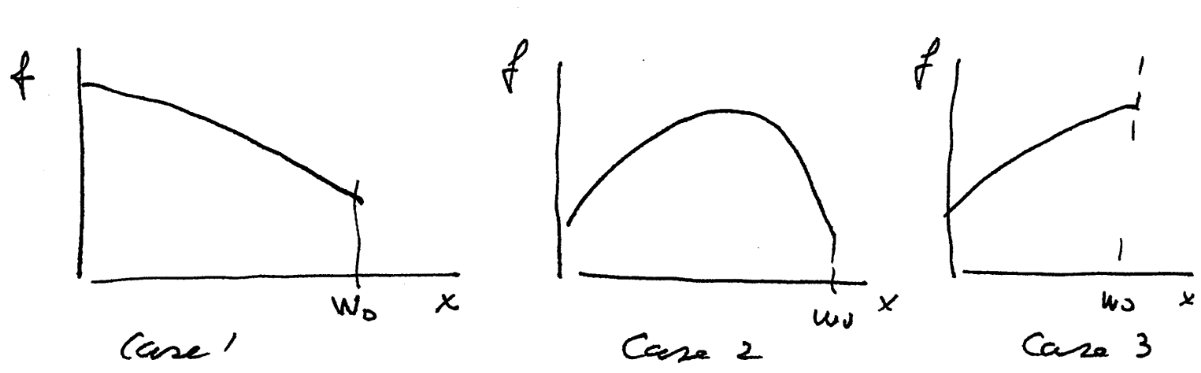
\includegraphics[width=0.8\textwidth]{L4-three-cases.png}
    \centering
\end{figure}
\end{frame}

\begin{frame}
\underline{Case 1}\\
\hfill \break
$\;\;\max\;f(x)$ at $x=0 \iff f'(x) \leq 0$\\
$\;\;\;\;\implies w=w_0$ and $u'(w) = u'(w_0) = \textit{constant}$\\
\begin{align*}
    \therefore \;\;\;\;&f'(0) = u'(w_0)E[z]\\
    &x=0 \iff E[z] \leq 0 \;\;\;\; [or\; E[z] \leq r_f]\\
    &x>0 \iff E[z] > 0\;\;\;\; \textit{independent of risk aversion}\\
\end{align*}
\underline{Case 3}\\
\[f'(w_0) = E[u'(w_0+w_0z)z] \geq 0\]
\end{frame}

\begin{frame}
\underline{Case 2:} Interior maximum at $f'(x^*)=0$\\
\[E[u'(w_0+x^*z)z] = 0\]
\hfill \break
given $u(\cdot)$ and the distribution of $z$, this can be solved for $x^*$.\\
\hfill \break
\begin{itemize}
    \item How does $x^*$ change with $w_0$? \textit{(see next page: implicit fn. thm.)}\\
\end{itemize}
\[\frac{dx^*}{dw_0} = -\frac{\partial f'/\partial w_0}{\partial f'/\partial x^*} = \frac{E[u''(w)z]}{E[u''(w)z^2]}\;\;\;\;\textit{(where $u''(w) < 0$)}\]
\[\therefore \;\; sign(\frac{dx^*}{dw_0}) = sign(E[u''(w)z])\]
\end{frame}

\begin{frame}
\underline{Recall:} Implicit Function Theorem\\
\begin{align*}
    &g(x,y) = 0\\
    &\frac{dx}{dy} = -\frac{\partial g / \partial y}{\partial g / \partial x}\\
\end{align*}
\end{frame}

\subsection{Relationships to Risk Aversion}
\begin{frame}
We will now show that \underline{decreasing} $A(w)$, that is $A'(w) < 0$, $\implies \frac{dx^*}{dw_0}>0$.\\
\hfill \break
Decreasing $A(w)$ implies
\begin{align*}
    -\frac{u''(w)}{u'(w)} = A(w_0+xz) &\leq A(w_0)\;\;\;\;\textit{for $z \geq 0$}\\
    \therefore \;\; u''(w_0+xz) &\geq -A(w_0)\cdot u'(w_0+xz)\\
\end{align*}
\end{frame}

\subsection{Unbounded Utility Functions}

\subsection{Multi-period Utility Functions}

%%%%%%%%%%%%%%%%%%%%%%%%%%%%%%%%%%%%%%%%%%%%%%%%%%%%%%%%%%%%%%%%%%%%%%%%%
%%%%%%%%%%%%%% TOPIC 5  Discrete Time Portfolio Selection %%%%%%%%%%%%%%%
%%%%%%%%%%%%%%%%%%%%%%%%%%%%%%%%%%%%%%%%%%%%%%%%%%%%%%%%%%%%%%%%%%%%%%%%%
\section{Discrete Time Portfolio Selection}
\subsection{Subsection}

%%%%%%%%%%%%%%%%%%%%%%%%%%%%%%%%%%%%%%%%%%%%%%%%%%%%%%%%%%%%%%%%%%%%%%%%%%%%%%%%%%%%%%%%
%%%%%%%%%%%%%% TOPIC 6  Mean-Variance Portfolio Choice and Asset Pricing %%%%%%%%%%%%%%%
%%%%%%%%%%%%%%%%%%%%%%%%%%%%%%%%%%%%%%%%%%%%%%%%%%%%%%%%%%%%%%%%%%%%%%%%%%%%%%%%%%%%%%%%
\section{Mean-Variance Portfolio Choice and Asset Pricing}
\subsection{Subsection}

\section{Math of Continuous Time Finance}
\subsection{Subsection}

\section{Continuous Time Diffusion Process}
\subsection{Subsection}

\section{Continuous Time Portfolio Selection}
\subsection{Subsection}

\section{Continuous Time Portfolio Selection and Asset Pricing}
\subsection{Subsection}

\section{Extended Model}
\subsection{Subsection}

\section{Consumption Based CAPM}
\subsection{Subsection}

\section{Introduction to Options}
\subsection{Subsection}

\section{Continuous Time Option Pricing}
\subsection{Subsection}

\section{The Options Approach to Valuing Risky Debt}
\subsection{Subsection}

\section{Stochastic Models of the Term Structure}
\subsection{Subsection}

\section*{References}
\begin{frame}[allowframebreaks]{References}
    \printbibliography
\end{frame}

\end{document}